\documentclass[12pt, a4paper]{article}

\usepackage[utf8]{inputenc}
\usepackage[T1]{fontenc}
\usepackage[brazilian]{babel}
\usepackage{mathptmx}
\usepackage{amsmath, amssymb}
\usepackage{graphicx}
\usepackage{booktabs}
\usepackage{geometry}
\usepackage{float}
\usepackage{setspace}
\usepackage{caption}

\geometry{top=3cm, bottom=2cm, left=3cm, right=2cm}
\setstretch{1.5}
\captionsetup{font=small, labelfont=bf, labelsep=endash}

\begin{document}

\begin{center}
    \Large\textbf{Relatório Intermediário de Benchmarking -- Cenário 3} \\[0.2cm]
    \large\textit{Análise Sequencial: Escalonamento Máximo (6 Núcleos) e o Colapso do Cache} \\[0.5cm]
    \normalsize\textbf{Projeto DataOps / UNIFEI} \\
    \small{\today}
\end{center}

\vspace{0.5cm}
\noindent\rule{\textwidth}{1pt}

\section*{1. Descrição do Cenário e Progressão Histórica}
Este documento consolida a terceira e última iteração da fase de testes focada no estrangulamento de \textit{hardware} (escalabilidade vertical). Nos relatórios precedentes, a mesmíssima base de dados fragmentada (3,1 milhões de registros distribuídos em 6.518 arquivos minúsculos - \textit{Tiny Segments}) foi submetida a processamentos sob rígidas restrições.

Em uma análise sequencial evolutiva, constatou-se que:
\begin{itemize}
    \item \textbf{No Cenário 1 (2 Núcleos):} O sistema agonizou em severo estrangulamento de \textit{I/O Overhead}, apresentando latências médias cruas na faixa dos $\sim$4.091 ms.
    \item \textbf{No Cenário 2 (4 Núcleos):} O provimento de paralelismo reduziu a ineficiência quase pela metade, estabilizando as leituras na casa dos $\sim$2.319 ms.
\end{itemize}

Neste \textbf{Cenário 3}, as travas do orquestrador Docker (\textit{Cgroups}) foram plenamente liberadas para a capacidade máxima do hospedeiro, alocando-se \textbf{6 núcleos lógicos} (3 \textit{threads} para o \textit{Broker} e 3 para o \textit{Historical}), acompanhados de 100 MB de alocação de \textit{Direct Memory}. O objetivo empírico é verificar se o \textit{hardware} de ponta consegue, por força bruta, superar o gargalo geométrico do disco.

\section*{2. Escalabilidade de Disco vs. O Colapso Absoluto do Cache}
Os resultados expressos na Tabela 1 demonstram a clássica escalabilidade teórica prevista pela Lei de Amdahl. A latência de varredura direta sobre os arquivos (\textit{Cold Start}) apresentou uma nova e expressiva melhoria, atingindo o teto de máxima eficiência desta arquitetura desorganizada com uma média global estabilizada em \textbf{$\sim$1.624 ms}.

\begin{table}[H]
\centering
\caption{Resultados do Cenário 3 - Capacidade Máxima (6 Cores) vs Fragmentação}
\vspace{0.2cm}
\begin{tabular}{@{}lcccc@{}}
\toprule
\textbf{Domínio da Consulta SQL} & \textbf{Cold (ms)} & \textbf{Warm (ms)} & \textbf{Otimização} & \textbf{Registros} \\
\midrule
    Bench 1 Serie Temporal & 1511.63 & 1639.02 & -8.43\% & 100 \\
    Bench 2 Alta Cardinalidade & 1756.32 & 1850.19 & -5.34\% & 50 \\
    Bench 3 Filtros Complexos & 1699.51 & 1613.72 & 5.05\% & 9 \\
    BI 1 ONS Infraestrutura & 1582.95 & 1590.50 & -0.48\% & 15 \\
    BI 2 FUNAI Terras Indigenas & 1548.98 & 1742.20 & -12.47\% & 10 \\
    BI 3 Defesa Civil Risco & 1646.85 & 1831.27 & -11.20\% & 81 \\

\bottomrule
\end{tabular}
\end{table}

Contudo, a grande descoberta analítica desta etapa reside na memória RAM. A Tabela revela que o aumento extremo de processamento simultâneo \textbf{agravou severamente o Paradoxo do Cache}. Das seis consultas estratégicas disparadas, cinco performaram substancialmente \textbf{pior} no \textit{Warm Start} do que no acesso cru ao disco. O painel da FUNAI (\textit{BI\_2}) alcançou absurdos \textbf{-12,47\% de degradação estrutural}.

\begin{figure}[H]
\centering
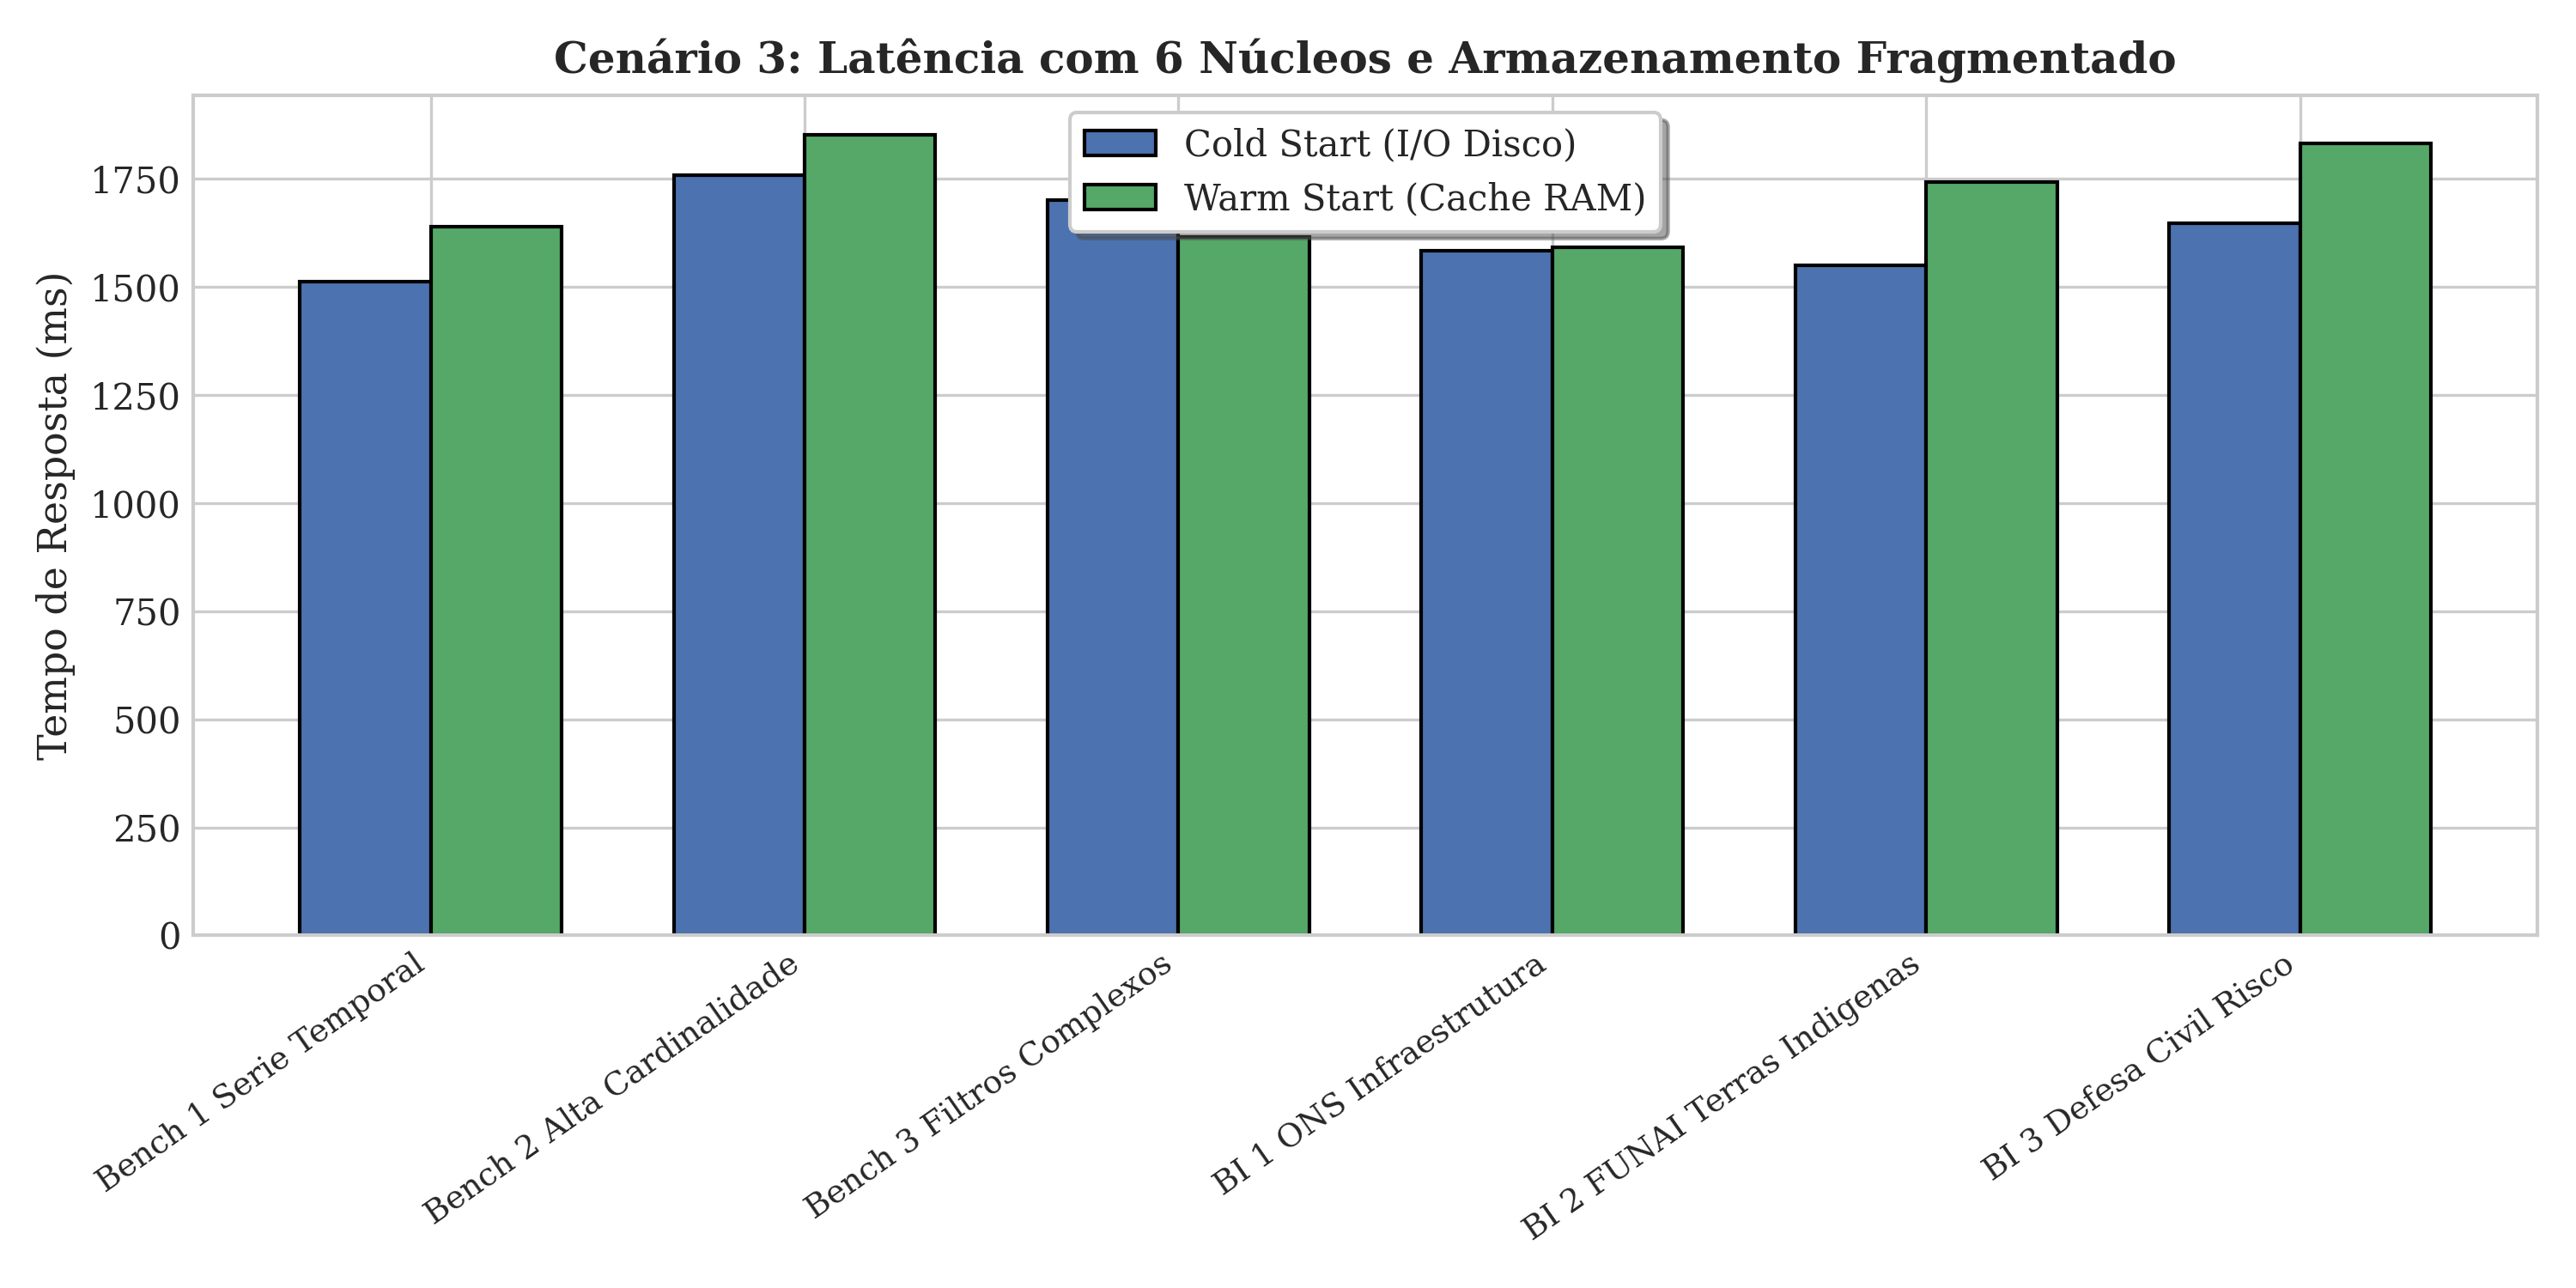
\includegraphics[width=0.9\textwidth]{fig_desemp_cenario3.png}
\caption{O recuo das latências brutas em contraposição ao congestionamento do cache.}
\end{figure}

\begin{figure}[H]
\centering
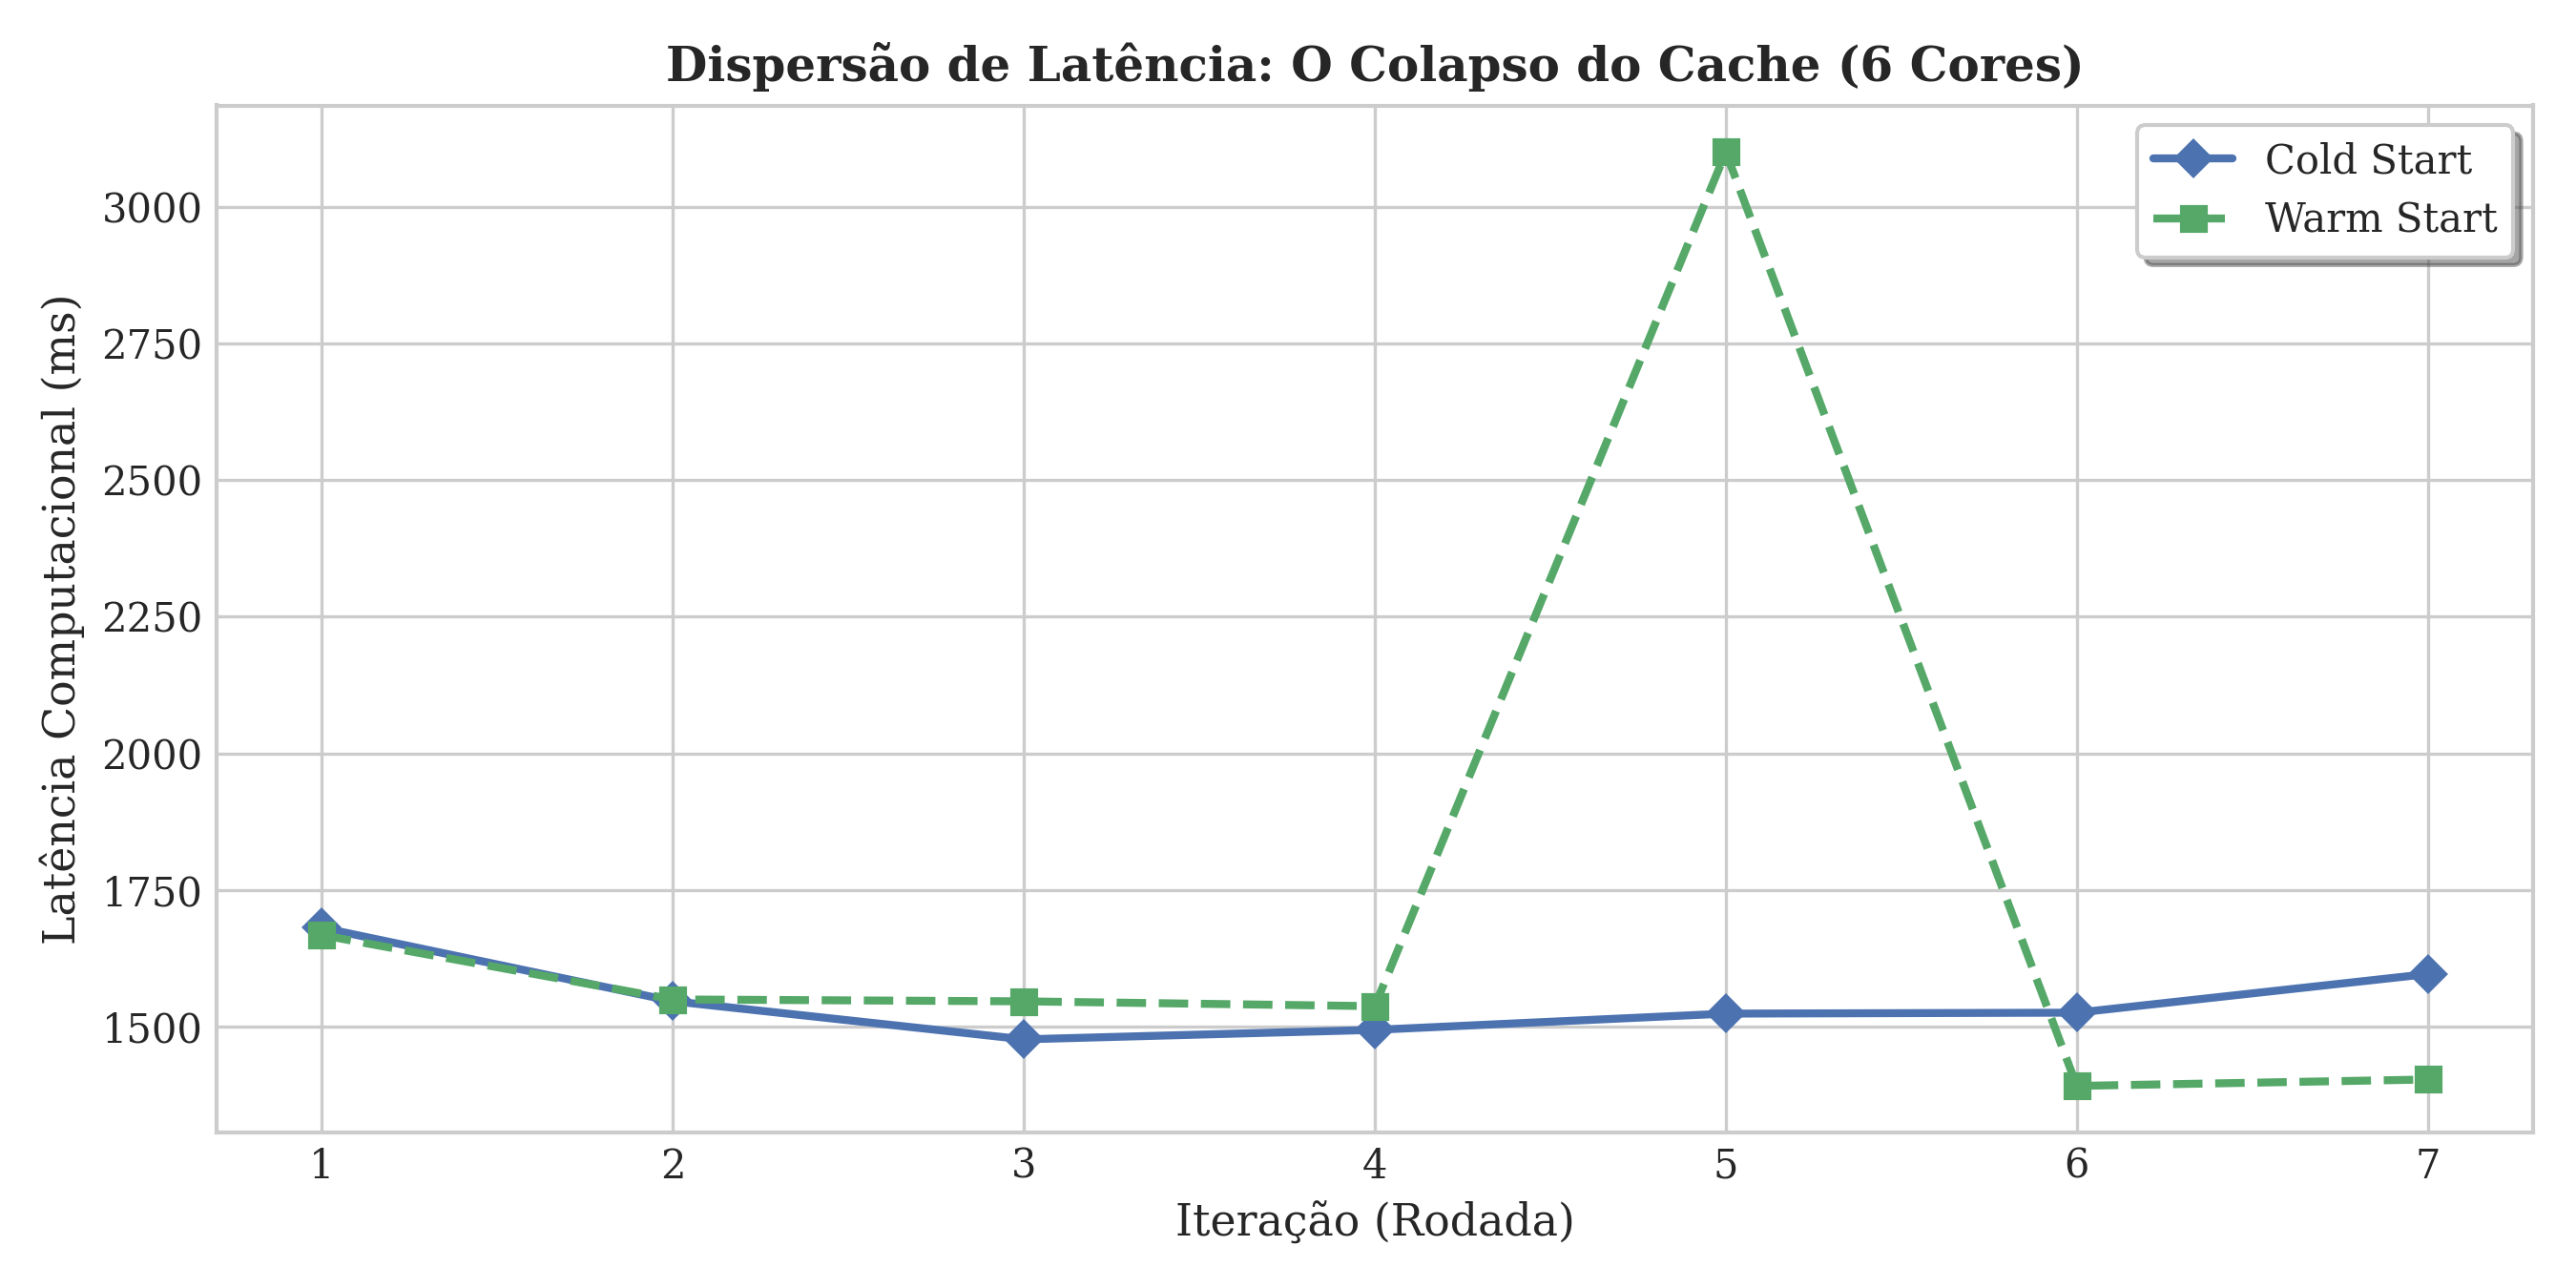
\includegraphics[width=0.8\textwidth]{fig_var_cenario3.png}
\caption{O exato momento (Consulta BI\_2) em que ler do disco torna-se mais vantajoso que o cache.}
\end{figure}

Isto fundamenta o fato de que, ao interceptar as \textit{queries}, o nó \textit{Broker} tenta varrer, unificar e agrupar na Memória Volátil as parciais herdadas dos 6.518 micro-arquivos. O custo logístico temporal desse "quebra-cabeça" afoga a ULA, superando amplamente o tempo que os 6 núcleos levariam simplesmente lendo o disco em paralelo.

\section*{3. Veredito da Fase de Escalabilidade}
A análise encadeada dos três cenários valida inequivocamente a premissa de que a escalabilidade puramente atrelada a \textit{hardware} possui um "teto de vidro" intransponível. A injeção de mais núcleos colapsou a estrutura interna de \textit{Cache}. Para romper a barreira técnica dos milissegundos e habilitar o pleno tempo-real (sub-segundos), abandona-se o \textit{Hardware Tuning} em prol do \textit{DataOps}, onde a próxima bateria de testes lidará com os dados plenamente compactados (\textit{Compaction}).

\end{document}
